\chapter{不確定性、埃倫費斯特定理與經典極限}

\section{線性哈密頓量留下的問題}

模型
\begin{equation}
H=cP
\label{eq:l10-linear-hamiltonian}
\end{equation}
之所以有用，是因為波包平移時形狀不變。但它也帶來一項嚴重警訊。動量可能為正，也可能為負，因此同一個公式會讓一個平面波具有正能量，另一個則具有負能量：
\begin{equation}
\psi_p(x)=e^{ipx/\hbar},
\qquad
E(p)=cp.
\end{equation}
如果任意多個物理粒子都能佔據負能量態，真空就不會是能量最低的狀態。真空可以產生正能量量子，同時將相抵的負能量交給新粒子，使總能量保持不變，卻讓真空能量無止境地降低。

\begin{classroomqa}
\audiencequestion{為什麼負能量分支不只是能量零點的一種奇特選擇？}
\lecturerresponse{把所有能量一律加上同一常數並無大礙；譜沒有下界則是另一回事。如果可以不斷布居能量更低的態，並由正能量粒子帶走相抵的能量，系統就沒有穩定的基態。穩定性要求能量相對於真空有下界。}
\end{classroomqa}

\begin{figure}[htbp]
\centering
\includegraphics[width=0.88\textwidth]{lecture_10_figure_01.png}
\caption{當\(p<0\)時，線性哈密頓量及其平面波本徵函數顯示出負能量分支。}
\lectureframe{00:04:35}
\end{figure}

狄拉克當年的解答適用於費米子。費米子遵守不相容原理：兩個全同費米子不能佔據同一個單粒子態。設想把所有負能量態都填滿。填滿之後，不相容原理便阻止其他費米子再進入這一區域。填滿的集合中若有一個空位，它便表現得像反粒子。

這個論證無法挽救負能量玻色子。任意多個玻色子都能佔據同一個態，因此負能量玻色子模式的佔據數可以無限增加。舊有的填滿海圖像，最好視為反粒子概念的歷史起點；現代量子場論描述粒子與反粒子時，不會把物理真空當成一片由可觀測的負能量電子構成的海。此處只需掌握一個較有限的結論：這個玩具哈密頓量並不是完整且穩定的粒子理論。

這個模型把以固定速率運動的費米子簡化成一維情形，也讓人聯想到狄拉克的想法曾與之相關的中微子問題。但它不能用來描述光子：光子是玻色子，不相容原理無法填滿並阻擋光子的負能量態。

\begin{classroomqa}
\audiencequestion{為什麼不相容原理能使費米子構造穩定，卻不能使玻色子構造穩定？}
\lecturerresponse{費米子態填滿後便會受到阻擋。玻色子態沒有佔據數上限，因此負能量玻色子模式仍會讓能量無止境地降低。}
\end{classroomqa}

\paragraph{課程進度}
這一季已建立了量子力學的許多基礎，也討論了幾個刻意簡化的系統，但應用還不多。尤其是，課程甚至還沒談到諧振子。這是課程進程的一個界線，並非終點：接下來會談相對論與場論，之後還得回到量子力學，研究諧振子及以它為基礎的其他架構。先前關於糾纏的討論引起了持續的興趣，也顯示沿著基礎一路探討是值得的。

有了這個脈絡，先前留下的問題便告一段落。接下來的重點是波函數、不確定性，以及量子演化與經典力學之間的關係。這裡要討論的不是最一般的演化方程，而是最初由Schr\"odinger寫下的特殊位置空間方程。

\section{波函數與完備對易座標}

對於直線上的單一粒子，位置空間波函數為
\begin{equation}
\psi(x)=\braket{x}{\psi},
\end{equation}
它表示在\(x\)附近找到粒子的振幅。動量空間波函數則為
\begin{equation}
\widetilde{\psi}(p)=\braket{p}{\psi}.
\end{equation}
兩者以不同的基底描述同一個抽象態，並由傅立葉變換相互轉換：
\begin{align}
\psi(x)
&=
\int_{-\infty}^{\infty}
\frac{dp}{\sqrt{2\pi\hbar}}\,
\widetilde{\psi}(p)e^{ipx/\hbar},
\label{eq:l10-fourier-forward}\\
\widetilde{\psi}(p)
&=
\int_{-\infty}^{\infty}
\frac{dx}{\sqrt{2\pi\hbar}}\,
\psi(x)e^{-ipx/\hbar}.
\label{eq:l10-fourier-inverse}
\end{align}

\begin{figure}[htbp]
\centering
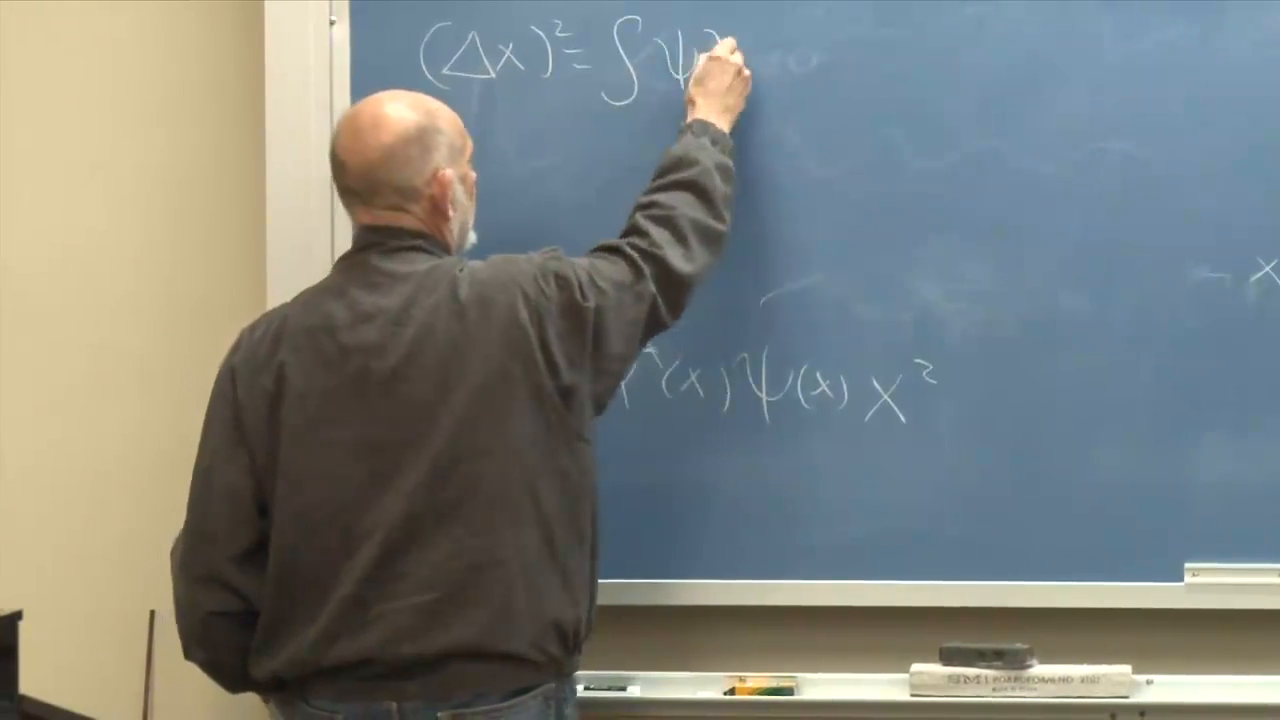
\includegraphics[width=0.88\textwidth]{lecture_10_figure_02.png}
\caption{位置空間與動量空間波函數，是同一個態在兩組不同連續基底上的投影。}
\lectureframe{00:09:05}
\end{figure}

在二維空間中，\(X\)與\(Y\)對易，因此可以用兩個座標標記共同本徵基底，波函數也就寫成\(\psi(x,y)\)。這種對易關係並非單由抽象公理所決定，而是對普通空間中量子力學的經驗描述之一。對於三維空間中的\(N\)個粒子，
\begin{equation}
\psi(\mathbf{x}_1,\ldots,\mathbf{x}_N)
\end{equation}
是定義在組態空間上的函數，而不是各自附著於每個粒子的三維波。因此，描述一個巨觀系統可能需要極大量的座標。

\begin{classroomqa}
\audiencequestion{不同空間座標的對易性是量子力學自動推導出的結果嗎？}
\lecturerresponse{不是。抽象架構容許許多種可觀測量代數。不同笛卡兒位置分量彼此對易，是普通空間中粒子量子力學的一項經驗性結構事實。}
\end{classroomqa}

可以對每個座標做傅立葉變換，得到以所有動量為變數的波函數；也可以只變換選定的變數。混合表象同樣成立，因為表象是基底的選擇，不會改變物理態。

\section{不確定性所量度的量}

不確定性原理最基本的形式，直接來自傅立葉對。動量確定的態是模長為常數的平面波，位置並未局域化。若要讓態在位置上高度局域，就需要許多動量分量。一般而言，傅立葉對中的一方越窄，另一方就越寬。

\begin{figure}[htbp]
\centering
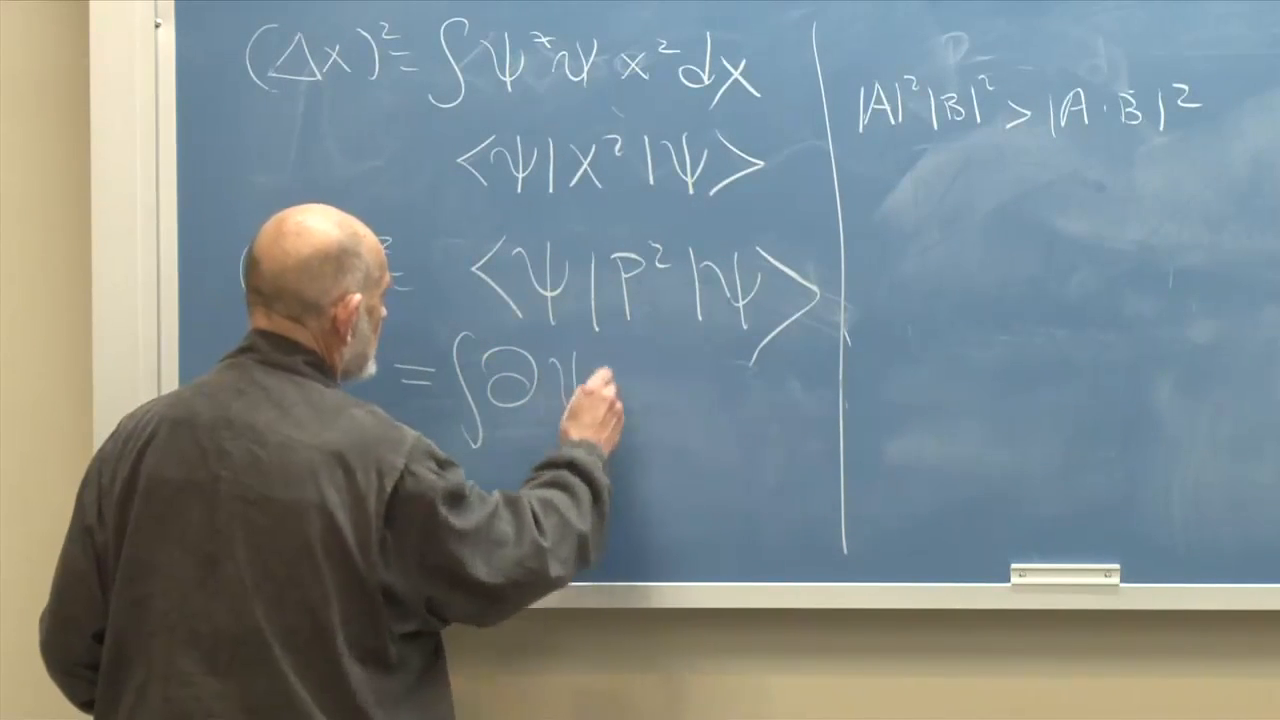
\includegraphics[width=0.88\textwidth]{lecture_10_figure_03.png}
\caption{位置分佈若要局域化，在互為倒數的動量表象中就必須是許多平面波的寬廣疊加。}
\lectureframe{00:14:45}
\end{figure}

要把這個說法定量化，先考慮一般可觀測量\(Q\)。它在歸一化態中的期望值為
\begin{equation}
\expect{Q}=\bra{\psi}Q\ket{\psi}.
\end{equation}
變異數為
\begin{equation}
(\Delta Q)^2
=
\expect{\bigl(Q-\expect{Q}\bigr)^2}
=
\expect{Q^2}-\expect{Q}^2.
\label{eq:l10-general-variance}
\end{equation}
不確定度\(\Delta Q\)則是變異數的正平方根。

考慮位置時，可以先平移原點，使\(\expect{X}=0\)。於是
\begin{equation}
(\Delta x)^2
=
\expect{X^2}
=
\int_{-\infty}^{\infty}
dx\,|\psi(x)|^2x^2.
\label{eq:l10-position-variance}
\end{equation}
正負貢獻在\(\expect{X}\)中會相消，在\(\expect{X^2}\)中則會相加。因此，機率分佈越寬，變異數也越大。

\begin{figure}[htbp]
\centering
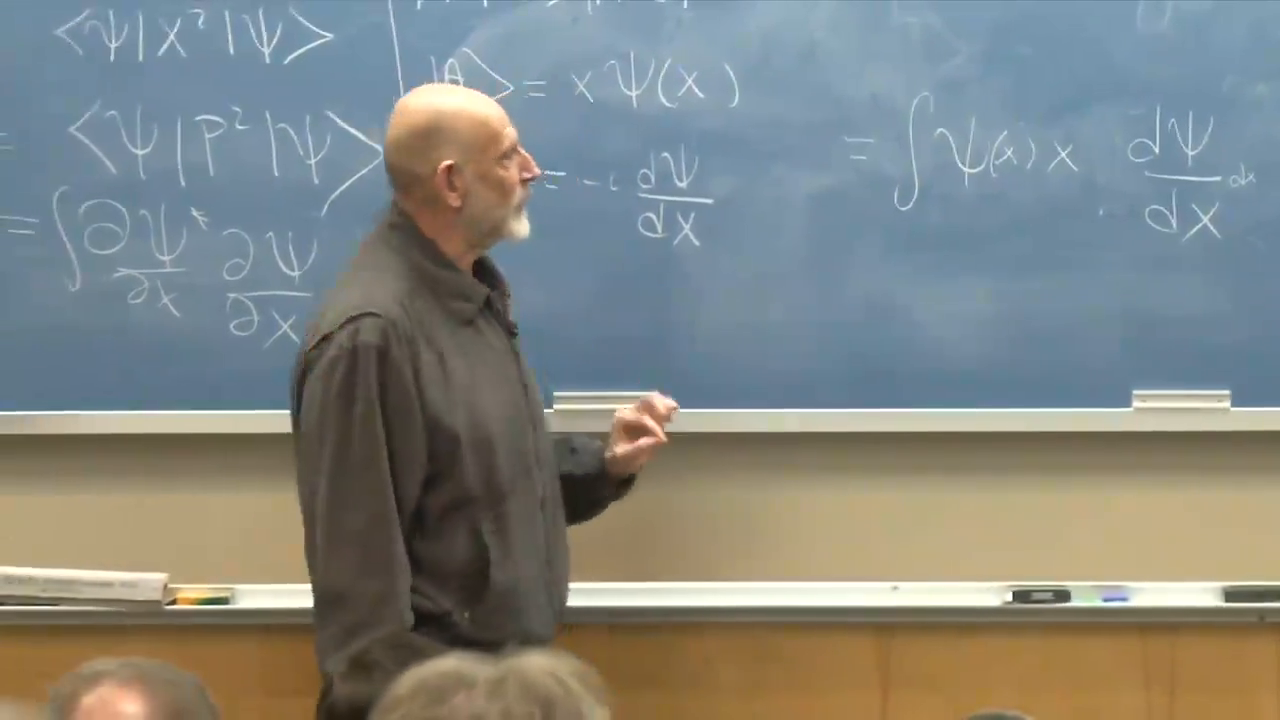
\includegraphics[width=0.88\textwidth]{lecture_10_figure_04.png}
\caption{將平均位置移至零後，位置變異數就是以機率加權的\(x^2\)積分。}
\lectureframe{00:20:50}
\end{figure}

\(\expect{X^2}\)與\(\expect{X}^2\)的差別至關重要。關於零對稱的分佈滿足\(\expect{X}=0\)；但只要分佈沒有完全集中在原點，就仍有\(\expect{X^2}>0\)。

動量變異數可以直接在動量空間中定義：
\begin{equation}
(\Delta p)^2
=
\int_{-\infty}^{\infty}
dp\,|\widetilde{\psi}(p)|^2
\bigl(p-\expect{P}\bigr)^2.
\end{equation}
不過，證明時改在位置空間處理較方便。將平均動量移至零，並使用
\begin{equation}
P=-i\hbar\frac{d}{dx},
\qquad
P^2=-\hbar^2\frac{d^2}{dx^2}.
\end{equation}
便有
\begin{equation}
(\Delta p)^2
=
\expect{P^2}
=
-\hbar^2
\int_{-\infty}^{\infty}
dx\,\psi^*(x)\frac{d^2\psi}{dx^2}.
\label{eq:l10-momentum-variance-second}
\end{equation}

\begin{classroomqa}
\audiencequestion{為什麼位置空間中的變異數公式前面有負號，變異數卻仍是正的？}
\lecturerresponse{乘上負號的積分值是非正的。分部積分會把一個導數移到\(\psi^*\)上，產生第二個負號，於是結果便成為絕對值平方的積分。}
\end{classroomqa}

若波函數在無窮遠處衰減得足夠快，
\begin{equation}
\int f\,g'\,dx
=
\left[fg\right]_{-\infty}^{\infty}
-
\int f'g\,dx,
\end{equation}
邊界項便會消失。將此式用於式~\eqref{eq:l10-momentum-variance-second}一次，可得
\begin{equation}
(\Delta p)^2
=
\hbar^2
\int_{-\infty}^{\infty}
dx\,
\frac{d\psi^*}{dx}
\frac{d\psi}{dx}
=
\hbar^2
\int_{-\infty}^{\infty}
dx\,
\left|\frac{d\psi}{dx}\right|^2
\geq 0.
\label{eq:l10-momentum-variance-positive}
\end{equation}

\begin{figure}[htbp]
\centering
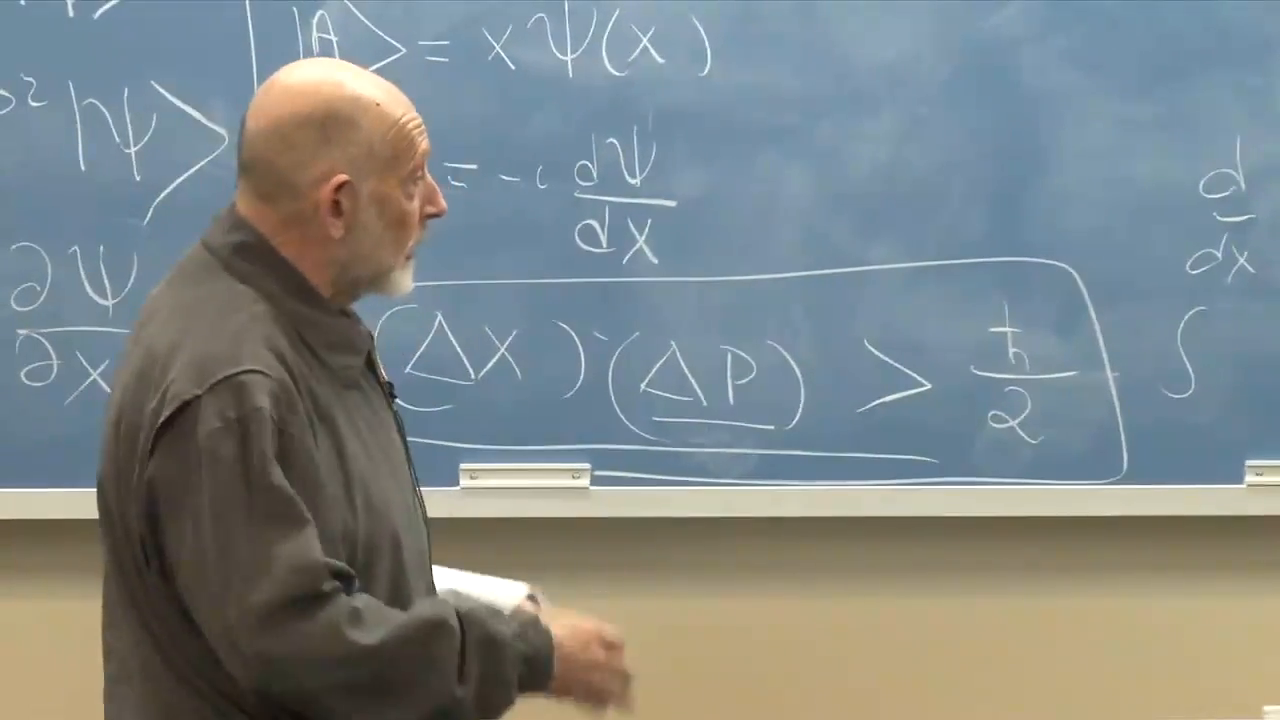
\includegraphics[width=0.88\textwidth]{lecture_10_figure_05.png}
\caption{分部積分把\(\expect{P^2}\)看似為負的表示式，化為明確非負的範數。}
\lectureframe{00:27:35}
\end{figure}

\begin{classroomqa}
\audiencequestion{位置與動量的平均值可以同時移至零嗎？}
\lecturerresponse{可以。平移波函數的自變數會改變\(\expect{X}\)；乘上平面波相位則會改變\(\expect{P}\)。這兩種操作會改變平均值，卻不改變各自的變異數，因此證明時可以把兩個變數都設為以平均值為中心。}
\end{classroomqa}

\section{不確定性下限}

這裡需要用到的數學工具是柯西--施瓦茨不等式。本講先從初等向量幾何來說明：兩個向量的內積等於兩者長度的乘積再乘上夾角的餘弦，因此內積的絕對值不會大於兩者長度的乘積。以希爾伯特空間的記號表示，
\begin{equation}
\braket{A}{A}\braket{B}{B}
\geq
\left|\braket{A}{B}\right|^2.
\label{eq:l10-cauchy-schwarz}
\end{equation}
這個不等式適用於任意維度的實或複向量空間。

\begin{figure}[htbp]
\centering
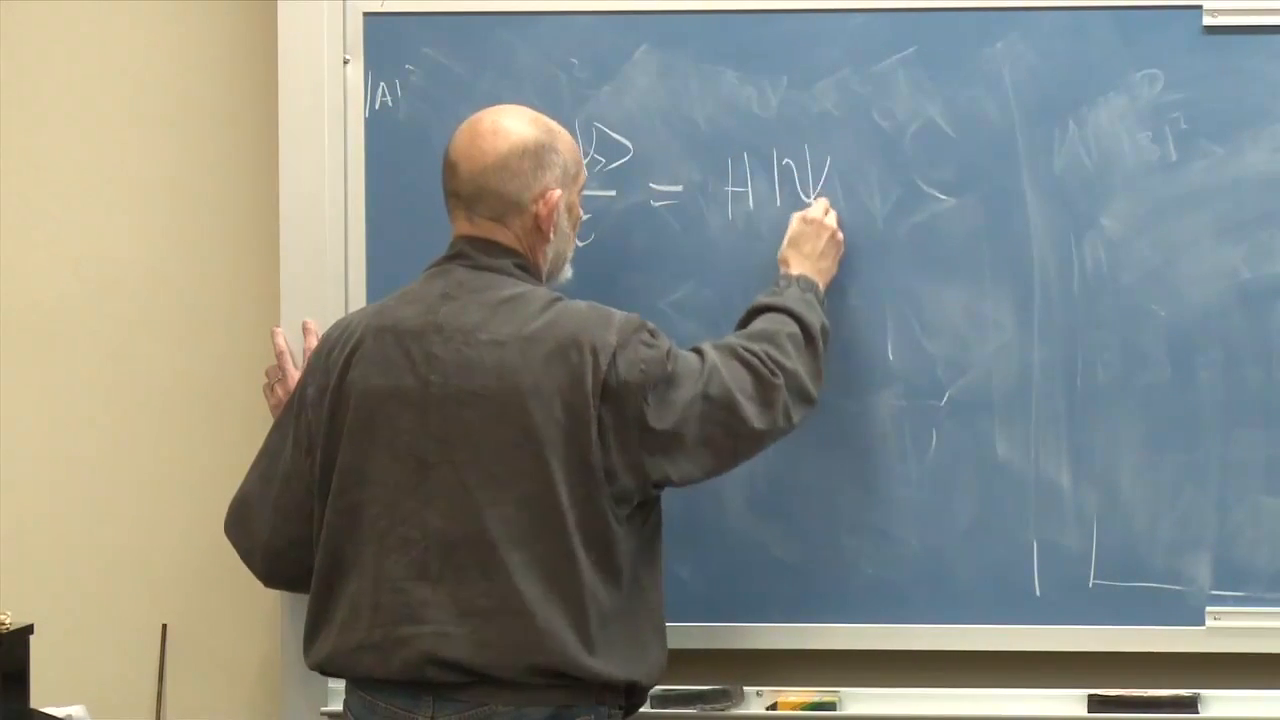
\includegraphics[width=0.88\textwidth]{lecture_10_figure_06.png}
\caption{幾何中的向量不等式改寫成希爾伯特空間中的柯西--施瓦茨界，供證明使用。}
\lectureframe{00:35:35}
\end{figure}

\begin{classroomqa}
\audiencequestion{這個不等式必須是嚴格不等式嗎？等號也可能成立嗎？}
\lecturerresponse{這裡是大於或等於。兩個希爾伯特空間向量線性相關時，等號成立。這個等號條件稍後會用來找出最小不確定度波包。}
\end{classroomqa}

將兩個變數都以平均值為中心，先依照黑板上的簡化證明，假設\(\psi(x)\)為實數。定義
\begin{equation}
\ket{A}=X\ket{\psi},
\qquad
\ket{B}=P\ket{\psi}.
\label{eq:l10-auxiliary-vectors}
\end{equation}
兩個向量的範數平方恰好就是兩個變異數：
\begin{equation}
\braket{A}{A}=(\Delta x)^2,
\qquad
\braket{B}{B}=(\Delta p)^2.
\end{equation}

\begin{figure}[htbp]
\centering
\includegraphics[width=0.88\textwidth]{lecture_10_figure_07.png}
\caption{輔助向量\(X\ket{\psi}\)與\(P\ket{\psi}\)將兩個變異數表示為希爾伯特空間中的範數。}
\lectureframe{00:44:40}
\end{figure}

剩下的內積為
\begin{align}
\braket{A}{B}
&=
\int_{-\infty}^{\infty}
dx\,
x\psi(x)
\left(-i\hbar\frac{d\psi}{dx}\right).
\end{align}
不等式中只會用到它的絕對值。由於\(\psi\)是實數，
\begin{equation}
\psi\frac{d\psi}{dx}
=
\frac{1}{2}\frac{d}{dx}\psi^2.
\end{equation}
因此，
\begin{align}
\left|\braket{A}{B}\right|
&=
\frac{\hbar}{2}
\left|
\int_{-\infty}^{\infty}
dx\,
x\frac{d}{dx}\psi^2
\right| \notag\\
&=
\frac{\hbar}{2}
\left|
-\int_{-\infty}^{\infty}
dx\,\psi^2
\right|
=
\frac{\hbar}{2},
\label{eq:l10-inner-product-half-hbar}
\end{align}
此處透過分部積分，從\(\psi^2\)與\(d x/dx=1\)中移去導數；邊界項消失，而最後一個等號則來自歸一化。

將式~\eqref{eq:l10-inner-product-half-hbar}代入柯西--施瓦茨不等式：
\begin{equation}
(\Delta x)^2(\Delta p)^2
\geq
\frac{\hbar^2}{4}.
\end{equation}
取正平方根後得到
\begin{equation}
\boxed{
\Delta x\,\Delta p
\geq
\frac{\hbar}{2}
}.
\label{eq:l10-uncertainty-principle}
\end{equation}

\begin{figure}[htbp]
\centering
\includegraphics[width=0.88\textwidth]{lecture_10_figure_08.png}
\caption{透過分部積分與歸一化，便得到位置與動量不確定性的精確下限。}
\lectureframe{00:50:55}
\end{figure}

假設\(\psi\)為實數只是為了簡化黑板上的推導，並非定理的限制。對一般複數態，令
\begin{equation}
\ket{A}=(X-\expect{X})\ket{\psi},
\qquad
\ket{B}=(P-\expect{P})\ket{\psi}.
\end{equation}
對易子決定了兩個輔助向量內積的虛部：
\begin{equation}
\operatorname{Im}\braket{A}{B}
=
\frac{1}{2i}\expect{[X,P]}
=
\frac{\hbar}{2}.
\end{equation}
由於\(|\braket{A}{B}|\)不小於其虛部的絕對值，同一個下限仍然成立。

\begin{classroomqa}
\audiencequestion{反覆分部積分時，邊界項究竟如何處理？}
\lecturerresponse{對於此處考慮的可歸一化波包，在\(+\infty\)與\(-\infty\)處出現的乘積都會消失。在有限的週期區間上，兩端的邊界項則會相消。運算子的定義域必須選得合適，才能確保這些條件成立；否則，形式上的推導就不成立。}
\end{classroomqa}

\begin{classroomqa}
\audiencequestion{等號在物理上真的可以達到嗎？還是這個下限只是一種估計？}
\lecturerresponse{可以達到。柯西--施瓦茨不等式要取等號，兩個輔助向量必須成比例。解出這個條件便得到高斯波包，也就是接下來要討論的最小不確定度態。}
\end{classroomqa}

\section{其他傅立葉共軛對}

時間與能量的不確定性關係，類似於位置與動量的關係；不過必須更謹慎地看待，因為在這裡，時間通常是演化參數，而非由一個普遍適用的自伴運算子表示的可觀測量。將態展開為能量本徵向量：
\begin{equation}
\ket{\psi(t)}
=
\int dE\,
\phi(E)e^{-iEt/\hbar}\ket{E}.
\label{eq:l10-time-energy-fourier}
\end{equation}
能量振幅與時間變化之間具有傅立葉關係。能量分佈越窄，態隨時間變化越慢，便無法形成時間上非常短促的脈衝；能量分佈越寬，則可能形成較短的到達時間包絡。

\begin{figure}[htbp]
\centering
\includegraphics[width=0.88\textwidth]{lecture_10_figure_09.png}
\caption{時間依賴性由能量本徵態組成，各態帶有相位\(e^{-iEt/\hbar}\)，這就構成了時間與能量關係的傅立葉基底。}
\lectureframe{00:53:40}
\end{figure}

\begin{classroomqa}
\audiencequestion{同一個證明可以直接套用在時間與能量上嗎？}
\lecturerresponse{倒數寬度的直觀想法仍然適用；傳遞中的波包便是一個有用例子：到達時間越短，所需的能量分佈就越寬。但運算子的說法較為微妙，因為在這種表述中，時間的角色與\(X\)並不完全相同。}
\end{classroomqa}

角度與角動量是旋轉運動中的另一組共軛量。在局部範圍內，兩者的傅立葉關係類似位置與動量。但從整體來看，角度具有週期性，必須另外謹慎處理。因此這裡只作類比，並未給出完整定理。

\begin{classroomqa}
\audiencequestion{位置與動量、時間與能量、角度與角動量，都是孤立的例子嗎？}
\lecturerresponse{不是。正則共軛變數一再以傅立葉對的形式出現。各組變數在定義域與週期性上的細節不同，但共同結構都是一方越局域，另一方就越分散。}
\end{classroomqa}

\section{位置空間中的Schr\"odinger方程}

現在回到動力學。抽象形式的定律是
\begin{equation}
i\hbar\frac{d}{dt}\ket{\psi(t)}
=
H\ket{\psi(t)}.
\label{eq:l10-abstract-schrodinger}
\end{equation}
對於質量為\(m\)、處於勢能\(V(X)\)中的粒子，取其哈密頓量為
\begin{equation}
H=\frac{P^2}{2m}+V(X).
\label{eq:l10-particle-hamiltonian}
\end{equation}
這裡採用經典力學中動能加勢能的形式，再檢驗量子演化是否能在適當條件下重現經典運動。

\begin{figure}[htbp]
\centering
\includegraphics[width=0.88\textwidth]{lecture_10_figure_10.png}
\caption{在含時Schr\"odinger方程中，哈密頓量作用於抽象態向量。}
\lectureframe{00:59:05}
\end{figure}

在位置表象中，\(P^2\)會變成二階微分算子。\(X\)的函數則以乘法作用：
\begin{equation}
\bigl(V(X)\psi\bigr)(x)=V(x)\psi(x).
\end{equation}
因此，
\begin{equation}
i\hbar\frac{\partial\psi(x,t)}{\partial t}
=
\left[
-\frac{\hbar^2}{2m}\frac{\partial^2}{\partial x^2}
+V(x)
\right]\psi(x,t).
\label{eq:l10-position-schrodinger}
\end{equation}

\begin{figure}[htbp]
\centering
\includegraphics[width=0.88\textwidth]{lecture_10_figure_11.png}
\caption{粒子的哈密頓量在位置表象中，成為動能所對應的二階微分項，加上以\(V(x)\)相乘的項。}
\lectureframe{01:03:05}
\end{figure}

\begin{classroomqa}
\audiencequestion{普通函數\(V(x)\)在什麼意義下是運算子？}
\lecturerresponse{選定位置基底後，\(X\)會以乘上\(x\)的方式作用。因此，夠規則的函數\(V(X)\)會在每個位置乘上對應的數值\(V(x)\)。它是否有用，得看接下來的動力學如何檢驗。}
\end{classroomqa}

為了計算期望值，先由方程~\eqref{eq:l10-position-schrodinger}解出波函數的兩個時間導數：
\begin{align}
\dot{\psi}
&=
\frac{i\hbar}{2m}\psi''
-\frac{i}{\hbar}V\psi,
\label{eq:l10-psi-dot}\\
\dot{\psi}^{\,*}
&=
-\frac{i\hbar}{2m}\psi^{*\,\prime\prime}
+\frac{i}{\hbar}V\psi^*.
\label{eq:l10-psi-star-dot}
\end{align}
第二行只是第一行的複共軛；把兩行都寫出來，便能清楚看出各項如何相消。

\section{波包中心的運動}

位置分佈的中心為
\begin{equation}
\expect{X}
=
\int_{-\infty}^{\infty}
dx\,\psi^*(x,t)\,x\,\psi(x,t).
\end{equation}
對時間微分：
\begin{equation}
\frac{d}{dt}\expect{X}
=
\int dx\,
\left(
\dot{\psi}^{\,*}x\psi
+
\psi^*x\dot{\psi}
\right).
\label{eq:l10-x-expectation-derivative}
\end{equation}
兩項互為複共軛。代入方程~\eqref{eq:l10-psi-dot}與\eqref{eq:l10-psi-star-dot}後，因為\(V(x)\)是實數，勢能項便會相消。再對動能項分部積分，可得
\begin{align}
\frac{d}{dt}\expect{X}
&=
\frac{1}{m}
\int dx\,
\psi^*
\left(-i\hbar\frac{\partial}{\partial x}\right)
\psi \notag\\
&=
\frac{\expect{P}}{m}.
\label{eq:l10-ehrenfest-x}
\end{align}

\begin{figure}[htbp]
\centering
\includegraphics[width=0.88\textwidth]{lecture_10_figure_12.png}
\caption{波包中心的變化率，化為動量期望值除以質量。}
\lectureframe{01:15:40}
\end{figure}

這個關係是精確的。整個代數推導沒有用到窄波包近似。

\begin{classroomqa}
\audiencequestion{這個推導在哪裡用到波包是單一窄峰的假設？}
\lecturerresponse{完全沒有用到。恆等式\(d\expect{X}/dt=\expect{P}/m\)對此哈密頓量定義域中的所有態都成立。只有在把\(\expect{X}\)詮釋為經典粒子的軌跡時，局域化才會派上用場。}
\end{classroomqa}

力學的另一部分涉及動量：
\begin{equation}
\expect{P}
=
\int dx\,
\psi^*
\left(-i\hbar\frac{\partial}{\partial x}\right)
\psi.
\end{equation}
對所有依賴時間的因子微分：
\begin{equation}
\frac{d}{dt}\expect{P}
=
-i\hbar
\int dx\,
\left(
\dot{\psi}^{\,*}\psi'
+
\psi^*\frac{\partial\dot{\psi}}{\partial x}
\right).
\label{eq:l10-p-expectation-start}
\end{equation}
先對其中一項分部積分，再代入兩個Schr\"odinger方程。動能項會相消；勢能項則合併為
\begin{equation}
\int dx\,
V(x)
\left(
\psi\frac{\partial\psi^*}{\partial x}
+
\psi^*\frac{\partial\psi}{\partial x}
\right)
=
\int dx\,
V(x)\frac{\partial}{\partial x}|\psi|^2.
\end{equation}
最後再做一次分部積分，將導數移到勢能上：
\begin{align}
\frac{d}{dt}\expect{P}
&=
-\int dx\,|\psi(x,t)|^2\frac{dV}{dx} \notag\\
&=
-\expect{V'(X)}
\\
&=
\expect{F(X)},\\
F(x)&=-V'(x).
\label{eq:l10-ehrenfest-p}
\end{align}

\begin{figure}[htbp]
\centering
\includegraphics[width=0.88\textwidth]{lecture_10_figure_13.png}
\caption{勢能項合併成全導數，於是得到\(d\expect{P}/dt=-\expect{V'(X)}\)。}
\lectureframe{01:30:45}
\end{figure}

方程~\eqref{eq:l10-ehrenfest-x}與\eqref{eq:l10-ehrenfest-p}就是這個哈密頓量的埃倫費斯特定理。它們是精確的量子力學恆等式，但期望值方程即使精確，也不等於經典軌道。

\section{經典近似從何處開始}

若把波包中心視為一個點，經典力學會要求
\begin{equation}
\frac{d}{dt}\expect{P}
\approx
F\!\left(\expect{X}\right).
\label{eq:l10-classical-center-force}
\end{equation}
然而，量子力學給出的是
\begin{equation}
\frac{d}{dt}\expect{P}
=
\expect{F(X)}.
\end{equation}
一般來說，
\begin{equation}
\expect{F(X)}
\neq
F\!\left(\expect{X}\right).
\label{eq:l10-force-nonlinearity}
\end{equation}

\begin{classroomqa}
\audiencequestion{如果兩個埃倫費斯特方程都精確成立，為什麼還不能證明每個量子態都遵循牛頓定律？}
\lecturerresponse{要讓波包中心遵循牛頓定律，力必須在中心位置計算。精確的量子方程則包含力在整個機率分佈上的平均值。對於處在力場緩慢變化區域的窄波包，兩者相同；但對任意態或非線性力而言，兩者未必相同。}
\end{classroomqa}

講課中的反例清楚顯示了兩者的差異。令\(F(x)=x^2\)，並選取一個由兩個等高窄峰組成的歸一化態，兩峰分別位於\(+a\)和\(-a\)附近。由對稱性可得
\begin{equation}
\expect{X}=0,
\qquad
F\!\left(\expect{X}\right)=0,
\end{equation}
然而
\begin{equation}
\expect{F(X)}
=
\expect{X^2}
\approx
a^2>0.
\end{equation}

\begin{figure}[htbp]
\centering
\includegraphics[width=0.88\textwidth]{lecture_10_figure_14.png}
\caption{對稱的雙峰波包若處於\(F(x)=x^2\)，平均位置處的力為零，但力的平均值不為零。}
\lectureframe{01:33:35}
\end{figure}

對於中心位於\(\bar{x}=\expect{X}\)的單一窄波包，將力展開：
\begin{equation}
F(X)
=
F(\bar{x})
+
F'(\bar{x})(X-\bar{x})
+
\frac{1}{2}F''(\bar{x})(X-\bar{x})^2
+\cdots.
\end{equation}
取期望值後，一次項便會消失：
\begin{equation}
\expect{F(X)}
=
F(\bar{x})
+
\frac{1}{2}F''(\bar{x})(\Delta x)^2
+\cdots.
\end{equation}
只要波包相較於力明顯變化的長度尺度夠窄，經典近似便可靠。

勢能中的尖銳特徵可能使波包分裂並造成散射。寬廣平滑的勢能通常能引導足夠局域化的波包，而不破壞它的單峰形狀；點狀障礙物、原子核，或尺度與波長相當的結構，則可能產生反射與繞射分量。

\begin{figure}[htbp]
\centering
\includegraphics[width=0.88\textwidth]{lecture_10_figure_15.png}
\caption{若勢能結構的尺度小於波包寬度或相關波長，相干波包就可能分裂成散射分量。}
\lectureframe{01:37:25}
\end{figure}

\begin{classroomqa}
\audiencequestion{什麼樣的勢能會妨礙波包呈現經典行為？}
\lecturerresponse{關鍵在於尺度，和道德好壞無關。若勢能特徵比波包尖銳得多，或尺度與波長相當，就會顯現波動性並產生散射。如果勢能在波包涵蓋的範圍內變化緩慢，力在該範圍內就近乎定值，波包中心因而遵循經典方程。}
\end{classroomqa}

質量也有影響。對於接近最小不確定度的波包，
\begin{equation}
\Delta x\,\Delta v
\sim
\frac{\hbar}{2m}.
\end{equation}
質量大時，波包可以兼具較小的空間寬度與適中的速度分散。因此，重物體通過巨觀尺度的勢能時，仍可能維持高度局域。輕粒子則更容易因微觀結構而擴散或繞射。這只是尺度上的論證，並不表示運動是否呈現經典行為只由質量決定。

\begin{classroomqa}
\audiencequestion{就這個意思而言，電子有可能大到足以近似呈現經典行為嗎？}
\lecturerresponse{可以，只要外場在電子波包的尺度上變化平緩。例如，在寬廣電容器極板之間，相干波包可以在一段足以觀察的時間內遵循經典加速度。到了原子核尖銳的庫侖場附近，同一個電子則會呈現明顯的散射。}
\end{classroomqa}

盧瑟福在1911年的散射實驗帶來了互補的啟示。{\proseunicodefont α}粒子遇上金原子核緊密集中的電荷分佈時，會被散射至大角度；這顯示正電荷集中在極小的區域。盧瑟福描述的是粒子束；量子力學描述的則是入射振幅及其散射分量。現代電子與光子散射實驗也利用同樣的尺度效應。

\begin{classroomqa}
\audiencequestion{這種波動性與尺度的關係只適用於物質粒子嗎？}
\lecturerresponse{不是。折射率相對於波長緩慢變化時，電磁波會遵循幾何光學。光柵間距若與波長相當，就會將波分散至不同方向。電子、{\proseunicodefont α}粒子、光子及其他量子激發，都遵循波長與結構尺度之間的這種關係。}
\end{classroomqa}

因此，經典極限不是額外加在量子力學上的另一條定律。精確的期望值方程本身已包含經典關係。當量子態維持局域化，而且哈密頓量變化平緩到足以使「對力取平均」近似等同於「在波包中心計算力」時，經典軌跡便會浮現。
